\renewcommand{\theequation}{\theenumi}
\begin{enumerate}[label=\arabic*.,ref=\thesubsection.\theenumi]
%\begin{enumerate}[1.]
\item Find the equations of two straight lines at a distance 3 from the origin and making an angle of $120 \degree$ with $OX$.
\item Find the equation of a straight line making an angle of $60\degree$ with $OX$ and passing through the point $\myvec{2\\-2}$.
Transform the equation to the form
\begin{equation}
\myvec{\cos\alpha &\sin \alpha}\vec{x} = p 
\end{equation}
\solution
Let the straight line pass through the point $\vec{A}=\myvec{2 \\-2}$ and makes an angle of 60$^{\circ}$ with x-axis.\\
So slope of the line, $m=\tan 60^{\circ}=\sqrt{3}$ and the direction vector  $\myvec{1 \\m} = \myvec{1 \\\sqrt{3}}$.\\\\
The vector form of the line passing through the point $\vec{A}=\myvec{2 \\-2}$ along the direction vector  $\myvec{1 \\\sqrt{3}}$ is given by:
\begin{align}
\vec{X}=\myvec{2 \\-2}+ \lambda_1\myvec{1 \\\sqrt{3}}
\end{align} 

The normal vector
\begin{align}
\vec{n}=\myvec{0 \quad -1\\1 \quad 0} \myvec{1 \\m} = \myvec{-\sqrt3\\ 1}
\end{align}
The equation of the line in terms of the normal vector is obtained as
\begin{align}
\vec{n^T}\myvec{x-A}  =0\\
\myvec{-\sqrt3\quad 1}x=\myvec{-\sqrt3\quad 1}A\\
\myvec{-\sqrt3\quad 1}x=\myvec{-\sqrt3\quad 1}\myvec{2 \\-2}\\
\myvec{-\sqrt3\quad 1}x=-2\sqrt{3}-2\\
\myvec{\sqrt3/2\quad -1/2}x=\sqrt{3}+1\\
\myvec{ cos 330^{\circ} \quad sin 330^{\circ}}x= 2.732
\end{align}
See Fig.     \ref{eq:solutions/2/2/2/myfig:1}

\begin{figure}[!ht]
 \begin{center}
  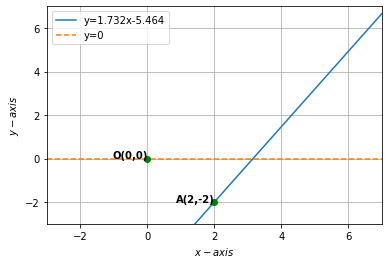
\includegraphics[width=\columnwidth]{solutions/2/2/2/assignment3_fig.png}
    \caption{This is the 2D diagram of the straight line passing through $\myvec{2 \\-2}$ and at an angle of 60$^{\circ}$ with the x axis }
    \label{eq:solutions/2/2/2/myfig:1}
    \end{center}
\end{figure}

\item Find the equation of the straight line that passes through the points $\myvec{2\\3}$ and $\myvec{3\\2}$. What is its inclination
to $OX$?
\item Find the equation of the straight line through the point $\myvec{5\\7}$ that makes equal intercepts on the axes.
\item Find the equations of the sides of a triangle whose vertices are $\myvec{2\\4}$, $\myvec{-4\\1}$ and $\myvec{2\\-3}$.
\item For the same triangle find the equations of the medians 
\item Find the equation of a straight line passing through the point $\myvec{2\\-3}$ parallel to the line $\myvec{4 & -1}\vec{x} + 7 =0$.
\item Find the intercepts on the axes made by a straight line which passes through the point $\myvec{3\\-1}$ and makes an angle
of $30\degree$ with $OX$.
\item Find the equation of the straight line through the points $\myvec{3\\-4}$, $\myvec{2\\3}$ and of the
parallel line through $\myvec{5\\2}$.
\item What is the distance from the origin of the line $\myvec{4 & -1}\vec{x} = 7$? Write down the equation of a parallel line at double the distance.
\item Find the equation of the straight line through the point $\myvec{3\\-4}$ parallel to the line joining the origin to the point
$\myvec{2\\-1}$.
\item Write down the equation of the straight line which makes intercepts 2 and -7 on the axes, and of the parallel line through
the point $\myvec{3\\-1}$.
\item Find the equations of the straight line joining the points $\myvec{3\\4}$, $\myvec{-2\\1}$ and of the parallel line through
the origin.
\item $ABC$ is a triangle and $\vec{A}, \vec{B}$ and $\vec{C}$ are the points $\myvec{2\\3}$, $\myvec{5\\-1}$ and $\myvec{-4\\2}$.  Find the equation
of the straight line through $\vec{A}$ parallel to $BC$.
\item Find the equation of a line parallel to $\myvec{2 & 5}\vec{x}=11$ passing through the middle point of the join of the points $\myvec{-7\\3}$, $\myvec{5\\-11}$.
\\
\solution
General equation of straight line is given by:\\
\begin{align}
    \vec{n}^T \vec{x} = c 
\end{align}   
\vspace{0.5 cm}
$\vec{n}$ will be same because both lines are parallel. \\
\begin{align}
    \vec{n} = \begin{pmatrix} 2  \\ 5 \end{pmatrix}
\end{align}
Passing through mid point $\vec{M}$ of $\vec{A}, \vec{B}$:
\begin{align}
  \vec{M} = \frac{ \vec{A} + \vec{B}}{2}
\end{align}
\begin{align}
    \vec{n}^T (\vec{x} - \vec{M}) = 0 \\
    \vec{n}^T \vec{x} = \vec{n}^T \vec{M} 
\end{align}

So, the mid point $\vec{M}$ is :
\begin{align}
   \vec{M} = \frac{\begin{pmatrix} -7  \\ 3 \end{pmatrix} + \begin{pmatrix} 5 \\ -11 \end{pmatrix}}{2}  = \begin{pmatrix} -1  \\ -4 \end{pmatrix}  \\
   \vec{n}^T \vec{x} =  \begin{pmatrix} 2 & 5 \end{pmatrix}\begin{pmatrix} -1  \\ -4 \end{pmatrix} = -22
\end{align}
So, the equation of line is :
\begin{align}
   \begin{pmatrix} 2 & 5 \end{pmatrix}\vec{x} = -22
\end{align}

\begin{figure}[t]
    \centering
    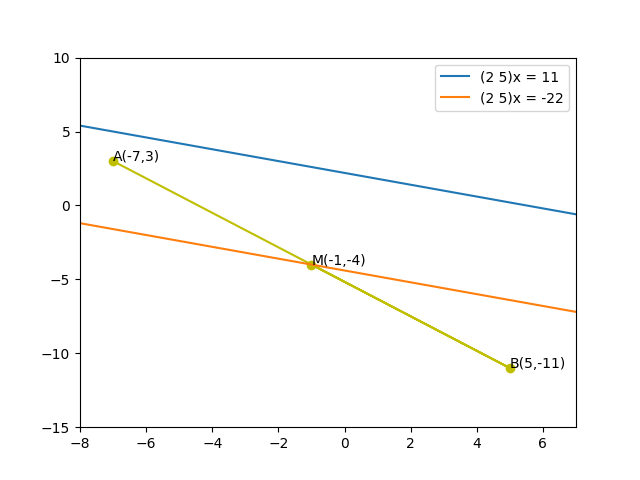
\includegraphics[width = \columnwidth]{./solutions/2/2/15/AI_assignment_2.png}
    \caption{Parallel Lines}
    \label{eq:solutions/2/2/15/fig:Lines}
\end{figure}


\item The base of a triangle passes through a fixed point $\myvec{f\\g}$ and the sides are bisected at right angles by the axes.  Prove that the locus
of the vertex is the line
\begin{equation}
\myvec{g & f}\vec{x} = 0
\end{equation}
\end{enumerate}
